%!TEX root = ./rules-working.tex
%LTeX: enabled=false

\rulechapter{Anti Aircraft Artillery (AAA) Units}

AAA unit counters are distinguished by class (H= heavy, M= medium, L= light) and gun type (85mm, 57mm, etc.).

Each counter is two sided. The “unfired” side has three rows of numbers on it. The “fired” side shows a gun silhouette and indicates the class and type of unit as well as its defense strength and spotting range. See the unit identification chart for an example of how to read the counter.

At the start of each game turn, the units are flipped to their unfired side. When they make an attack, they're flipped to the fired side as a reminder that they've been used.

\paragraph{Maximum Effective Range/Altitude.} There are three range categories for each AAA unit; short, medium and long. The maximum range in hexes for each category is indicated by the top row of three numbers on the unit's unfired side. When figuring range, each two full altitude levels up equals one hex of range. If the target is on a hexside, treat it as being in the hex closest to the AAA unit.

AAA units also have a maximum effective altitude. The bottom left hand number on the unfired side of the unit lists its maximum effective altitude. This is the maximum number of levels above the unit that a target can be fired at.

Example: The range to an aircraft three hexes away from, and ten altitude levels above a AAA unit is eight. Even if a AAA unit has an effective range better than eight, it may not hit the above target unless its maximum effective altitude is also ten or greater.

\paragraph{AAA Roll To Hit.} 
%!TEX root = ../rules-working.tex
%LTeX: enabled=false
\addedin{1C}{1C-tables}{
\begin{onecolumntablefloat}
\begin{onecolumntable}
\tablecaption{table:aaa-unit-attack-modifiers}{AAA Unit Attack Modifiers}

\begin{tabularx}{0.8\linewidth}{lL}
\toprule
Modifier&Condition\\
\midrule
\plus{1}    &If AAA unit D damaged.\\
\plus{2}    &If AAA units 2D damaged.\\
\plus{1}    &If firing into Sun clutter.\\
\plus{2}    &If integral FCR jammed or not used.\\
\minus{1}   &If FCR-A unit in use.\\
\minus{2}   &If FCR-B or C unit in use.\\
\minus{3}   &If FCR-D unit in use.\\
\bottomrule
\end{tabularx}
\end{onecolumntable}
\end{onecolumntablefloat}
}

%!TEX root = ../rules-working.tex
%LTeX: enabled=false
\addedin{1B}{1B-tables}{
\begin{onecolumntablefloat}
\begin{onecolumntable}
\tablecaption{table:djm-and-chaff-effects-against-fcrs}{DJM and Chaff Effects Versus FCRs.}

\begin{tabularx}{0.8\linewidth}{CCCCCC}
\toprule
DJM Type&Chaff PPL \#&\multicolumn{4}{c}{FCR Type}\\
&&LF&HF&VF&MW\\
\midrule
A   &1      &\plus{1}   &\plus{1}   &\plus{0}   &\plus{0}   \\
B   &2--3   &\plus{2}   &\plus{2}   &\plus{1}   &\plus{0}   \\
C   &4--5   &\plus{2}   &\plus{2}   &\plus{2}   &\plus{1}   \\
D   &6      &\plus{2}   &\plus{2}   &\plus{2}   &\plus{2}   \\
\bottomrule
\end{tabularx}
\end{onecolumntable}
\end{onecolumntablefloat}
}

The three numbers appearing in the middle row of the unfired side of the unit are the base “Roll to hit” numbers corresponding to each of the three effective ranges. When a AAA attack is announced against an aircraft, these numbers are referenced and a die is rolled and modified \changedin{1B}{1C-tables}{as appropriate}{according to Tables \ref{table:aaa-unit-attack-modifiers} and \ref{table:djm-and-chaff-effects-against-fcrs}}. If the result is less than or equal to the Roll to Hit number, a hit is achieved.

Note:  If the roll to hit number is a zero, this means the gun cannot normally hit the target without the help of die roll modifiers which reduce the roll to zero or less.

\paragraph{Attack Rating.} The middle number on the bottom row of the unfired side of the AAA unit is its listed attack rating. AAA units have variable attack ratings however. The listed attack rating represents the maximum allowed attack rating that the unit can have. Each time a hit is achieved through aimed or plotted fire, roll the die again. If the result is greater than or equal to the AAA unit's maximum rating, then the rating is used in conjunction with the damage tables. If the second roll was less than the maximum rating, then the number on the die roll is used for the unit's attack rating. Once the attack rating is determined, roll for damage normally.

Chance hits achieved in barrage fire zones or plotted fire zones are always resolved with an attack rating of 1 or 2 (depending on gun size), regardless of the unit's maximum allowed attack rating.

\paragraph{AAA Damage.} Damage to aircraft is determined using the Damage tables as per Rule \ref{rule:aircraft-damage-resolution}.

\section{AAA Unit Fire Modes}

AAA attacks can occur in three ways; through AIMED fire, BARRAGE fire, or PLOTTED fire. Each is a distinct mode and eligible AAA units may use only one of these modes each turn.

Light AAA units may use only aimed or barrage fire. Medium AAA units may opt for any mode. Heavy AAA units may use only aimed or plotted fire. AAA units desiring or required to use barrage or plotted fire modes are designated in the AAA Interaction Phase of the game-turn. All other AAA units are considered to be in the aimed fire mode.

\subsection{Aimed Fire Mode}

Aimed fire represents the deliberate engagement of a single aircraft by a AAA unit. All AAA units may use this mode.

\paragraph{Aimed Fire Procedure.} Aimed fire attacks are announced and resolved during the Flight Phase. As an enemy aircraft is moved, unfired AAA units using aimed fire may track and attack the aircraft. Only the currently moving aircraft is eligible to be fired on. Aimed fire may not be used against aircraft which have not yet moved or which have already completed their moves that game turn.

The aimed fire attack may be made the instant that tracking is completed, or anytime thereafter during the target's move. When an aimed attack is announced, the target's flight is temporarily halted and the attack is resolved. Damage effects are applied immediately, then the target completes its move (if able).

\paragraph{Tracking.} To track a target, the AAA unit must have a line of sight to it, and the target must be within one and a half times the AAA unit's maximum effective range. Tracking begins when the AAA unit declares it is doing so. Tracking is considered complete for manually aimed guns the moment a tracked aircraft expends FPs equal to 1/2 or more of its speed (round fractions up) in the AAA unit's line of sight. Tracking is considered complete for radar directed guns the moment FPs equal to 1/3 the target's speed (round fractions up) are expended.

Exception: Heavy AAA units must track a target for two thirds (2/3) its speed in FPs (round fractions up) before firing whether manual or radar guided.

Tracking may be carried over from turn to turn but must begin anew after each aimed shot taken. AAA units may still only fire once per game-turn.

\paragraph{Switching targets.} AAA units planning to use aimed fire which track but do not shoot at one aircraft in a game turn may switch to and track subsequent aircraft that move. Each switch within a game turn however, carries a cumulative \plus{1} modifier to the aimed fire die roll.

\subsection{Barrage Fire Mode}

%!TEX root = ../rules-working.tex
%LTeX: enabled=false

\addedin{1B}{1B-figures}{

\begin{onecolumnfigure}

\begin{fitheight}{5.2\standardhexwidth}
\begin{tikzpicture}
    \setfiguresize{-2.5}{-2.6}{+2.5}{+2.6}
    \drawevenhexgrid{-2}{-2}{5}{5}
    \begin{scope}[xscale=\hexxfactor,ultra thick,black]
        \draw 
            (-1.333,+0.000) -- 
            (-1.667,+0.500) -- 
            (-1.333,+1.000) --
            (-0.667,+1.000) --
            (-0.333,+1.500) --
            (+0.333,+1.500) --
            (+0.667,+1.000) -- 
            (+1.333,+1.000) --
            (+1.667,+0.500) --
            (+1.333,+0.000) --
            (+1.667,-0.500) --
            (+1.333,-1.000) --
            (+0.667,-1.000) --
            (+0.333,-1.500) --
            (-0.333,-1.500) --
            (-0.667,-1.000) --
            (-1.333,-1.000) --
            (-1.667,-0.500) --
            cycle;
    \end{scope}
    \node at (0,0) [align=center] {Target\\Hex};
\end{tikzpicture}
\end{fitheight}

\figurecaption{figure:aaa-zone}{AAA Barrage and Plotted Fire Zone of Effect.}

\end{onecolumnfigure}
}


When faced with multiple attackers, AAA gunners often resort to the simple expedient of filling the sky in and around their position with large amounts of “lead” (bullets) in the hope that an aircraft will run into one. This unaimed form of panic fire can be effective due to the sheer density of fire.

Only Light and Medium AAA units may use barrage fire. Designate during the AAA Interaction Phase which units will use barrage fire by placing a barrage marker on them.

\paragraph{Zone Of Effect.} Barraging units have a zone of affect about them for the entire game turn. This zone consists of the hex the unit is in plus the six adjacent hexes and the hexsides forming them,\addedin{1B}{1C-figures}{ as shown in Figure \ref{figure:aaa-zone},} from the ground level up to the maximum altitude above the unit the weapon can reach.

Aircraft which fly into this zone of effect (whether friendly or enemy) must check for chance hits. Roll the die once \changedin{1C}{1C-apj-36-errata}{for each FP expended}{after each FP expended that ends} in the zone. On a roll of 1 a chance hit occurs. Resolve this hit immediately using an attack rating of 1 for Lt.\ AAA and small arms, and a 2 for Medium AAA on the damage tables. If more than one zone of effect overlaps a hex, each zone is rolled for separately.

\paragraph{Ammo Effects.} AAA units which use this tactic run out of ammo at the end of the game-turn. Flip the barrage marker to the out of ammo side to reflect this. They may not fire again until they are resupplied. During the End Of Turn Admin Phase of each game-turn (including the current one) roll one die for each out of ammo unit. On a 2 or less, it is resupplied.

\paragraph{Non-AAA Unit Anti-Aircraft Fire.} Some non-AAA ground units and naval units are capable of using barrage fire against aircraft. Armored vehicle units, vehicular HQ units, regular infantry platoons and infantry headquarter all have barrage fire capability due to small arms fire. Infantry small arms fire reaches to two altitude levels above the unit, while vehicular small arms fire reaches to three levels above (greater proportion of machine guns). In all respects small arms fire is treated as barrage fire except that non-AAA units never run out of ammo.

\subsection{Plotted Fire Mode}

Plotted fire represents the use of preplanned area flak barrages. Plotted fire creates a zone of effect which remains in play for one whole game-turn. Only Medium and Heavy AAA units may use plotted fire.

\paragraph{Plotted Fire Procedure.} During the AAA Interaction Phase, a target hex and altitude is secretly noted for each AAA unit using plotted fire.

In the Ground Unit Interaction Phase of the game-turn, the target hex and altitude are revealed. A plotted fire zone of effect is considered to now exist in the target hex and the six adjacent hexes and any hexsides that form them\addedin{1B}{1C-figures}{ as shown in Figure \ref{figure:aaa-zone},} this at the plotted altitude, plus or minus two levels. \addedin{1C}{1C-apj-36-errata}{It is possible for parts of a plotted fire zone to extend beyond the normal maximum range/altitude of the gun.}

Any and all aircraft, friendly or enemy, that are caught in the plotted fire zone are immediately subject to one attack. Resolve the attack as if by aimed fire but with an additional \plus{1} modifier to the hit roll. If plotted fire cannot normally hit due to modifiers, the target is not attacked but is still subject to chance hits during its movement next game-turn.

\paragraph{Plotted Fire Marker.} The plotted fire zone's location is noted by placing an area fire marker in the plotted target hex. The fire zone remains in effect from the current Ground Unit Interaction Phase to the next turn's Ground Unit interaction Phase. Any aircraft which later expends flight points in a plotted fire zone, must check for chance hits  \changedin{1C}{1C-apj-36-errata}{for each FP so expended}{after each FP expended that ends in the zone}, as for barrage fire. \addedin{1C}{1C-apj-36-errata}{When rolling for chance hits from plotted fire zones, all fire at the same hex/altitude counts creates one zone, and therefore results in one die roll, but the concentrated fire die roll modifiers are used. Plotted fire zones that overlap but are not targeted at the same hex/altitude create separate die rolls for the main attack and also for chance hits.}

\paragraph{Concentrated Fire.} More than one AAA unit of the same or different types (heavy or medium) may be plotted to the same target hex/altitude. In this case, only one attack per plane caught in the zone is still allowed. Use the least accurate AAA unit's to hit numbers but allow a \minus{1} to hit modifier for each firing unit over one. If a hit is scored, the highest maximum attack rating of all the AAA units involved is utilized to determine actual attack rating.

\addedin{1C}{1C-apj-23}{
\paragraph{Plotted Fire Damage.}
\changedin{1C}{1C-apj-36-errata}{Chance hits of Heavy AAA in a plotted fire zone have an attack rating of 2.}{If at least one Heavy AAA unit contributed to the \changedin{2B}{2B-heavy-barrage-fire}{barrage}{plotted-fire} zone, use an attack rating of 2 for chance hits.} Regular hits achieved when plotted fire is revealed and resolved use the regular die roll procedure to determine the attack rating.
}

\section{Fire Control Radars (FCRs)}

FCRs are used to increase the accuracy of AAA guns. Some AAA units may have built in “Integral” FCRs and others may be allowed to use “add on” FCRs.

\paragraph{Integral FCRs.} AAA units that have integral fire control radars are indicated by an “R” or “W” in the bottom right corner of the unfired side of the unit counter. These units have the radar's effects already figured into the to hit numbers. If an integral radar is jammed or turned off for any reason, a +2 to hit modifier is applied to the unit.

\paragraph{Add-On FCRs.} Other non-mobile AAA units may be linked to an FCR at the start of play by stacking an FCR counter on the AAA unit. Only Medium and Heavy units of 30mm size or greater may utilize add-on FCRs. The AAA unit stacked with the FCR automatically gets the FCR's to hit modifier bonus as long as the radar is not jammed or turned off and a line of sight exists to the target aircraft. An FCR can only be linked to one AAA unit at a time and this is designated at the start of a game. FCRs cannot be switched to other AAA units even if in the same hex within the course of a game.

\paragraph{Weather Effects (Advanced Rule \ref{rule:night-and-weather}).} Add on FCRs are all weather capable and allow the AAA unit to track and fire on enemy aircraft at night and in adverse weather even if not visually sighted.

Integral FCRs marked by a “W” are all weather capable and function as above. Integral FCRs marked by an “R” are range only radars and function only against visually sighted targets.

\section{AAA and Aircraft Sighting}

\paragraph{Sighting Restrictions.} AAA units and small arms capable ground units are assumed to automatically sight aircraft and may begin tracking them at any point in the Flight Phase in which the aircraft becomes or is visible to them based on line of sight restrictions and the following limitations:

\begin{itemize}

    \item No aircraft may be visually sighted beyond four times its visibility number.

    \item No aircraft in TFF may be visually sighted by units at the same or lower altitude until within 12 hexes of range (assuming a line of sight exists).

    \item In HAZE, (see rule \ref{rule:night-and-weather}), no aircraft may be sighted beyond twice its visibility number in range.
    
    \itemdeletedin{1C}{1C-apj-23-errata}{AAA units not using an FCR may not fire on units, althoigh they may track them, until withing twice the aircraft's visibility number in range.}

\end{itemize}

\trainingnote{
You may now play Training scenario five and all scenarios except those involving Surface to Air Missiles (SAMs)!
}

\begin{advancedrules}

\section{Aircraft Jinking}

%!TEX root = ../rules-working.tex
%LTeX: enabled=false
\addedin{1B}{1B-tables}{
\begin{onecolumntablefloat}
\begin{onecolumntable}
\tablecaption{table:jinking}{Jinking Versus AAA}

\begin{tabularx}{0.9\linewidth}{lL}
\toprule
AAA Range&Maneuvering Required\\
\midrule
Short           & BT turns, snap turns, or rolls, or VIFF maneuvers.\\
Medium and Long & As above plus HT turns.\\
\bottomrule
\end{tabularx}
\begin{tablenote}{0.9\linewidth}
Die roll to evade hit:

\begin{itemize}
    \item \plusafter{6} if AAA not FCR aimed
    \item \plusafter{8} if AAA is FCR aimed
\end{itemize}

Apply aircraft size modifier from ADC to this die roll.
\end{tablenote}

\end{onecolumntable}
\end{onecolumntablefloat}
}


Maneuvering aircraft are more difficult targets for AAA guns. A good strike pilot will develop his own pattern of jinks to fool enemy gunners. \addedin{1B}{1C-tables}{The rules for jinking are described here and summarized in Table \ref{table:jinking}.}

\paragraph{Jinking Parameters.} To be considered jinking, an aircraft must meet one of the following parameters:

\begin{itemize}
    \item If the AAA range was short; the aircraft must be in a BT or greater turn rate or just have faced due to a turn at BT or greater rate; or the aircraft must be prepping for or just have executed a roll maneuver of any sort, or VIFF maneuver of any sort.

    \item If the AAA range was medium or long; the aircraft must be in an HT or greater turn rate or just have faced due to an HT or greater turn rate or must be prepping for, or executing maneuvers as above.
\end{itemize}

\addedin{1C}{1C-apj-23-errata/1C-apj-36-errata}{When jinking turns may not be stretched out with extra FPs before changing facing. Reversing the angle of bank when going directly from one turn to another still constitutes jinking if the aircraft is shot at while reversing.} \addedin{1C}{1C-apj-36-errata}{In this case, the new turn need not qualify for jinking.}

\paragraph{Jinking Effect.} A jinking aircraft which is hit by AIMED or PLOTTED AAA fire is allowed an immediate die roll to negate the hit; meaning the gunners actually missed. Roll a die before any attack rating or damage is determined.

If the roll is a 6 or more against manually directed guns, or 8 or more against radar directed guns, the hit is nullified and becomes a miss. Consider it a paint scorching “Close, but no cigar” shot. The aircraft size modifier is applied to this roll. Jinking aircraft taking a Chance hit from a barrage or plotted fire zone, do not get a nullifying die roll.

\section{Heavy AAA Unit Facing}
\label{rule:heavy-aaa-unit-facing}

Heavy AAA units, due to the size of the guns they represent, must be set up facing a specific hexside or juncture. This facing can be changed by up to 60° each game-turn in the AAA planning phase. Consider the top of the counter to be the front of the unit. Heavy AAA units may only shoot at aircraft or do plotted fire in their field of fire which consists of their \arcplus{180} arc, relative to their facing (front), and their own hex (straight up).

\section{Solitaire and Random AAA Fire}

%!TEX root = ../rules-working.tex
%LTeX: enabled=false
\addedin{1B}{1B-tables}{
\begin{onecolumntablefloat}
\begin{onecolumntable}
\tablecaption{table:random-aaa}{Random AAA Fire.}

\begin{tabularx}{0.9\linewidth}{lL}
\toprule
\multicolumn{2}{c}{Aimed Fire Attempt Roll}\\
\midrule
Range to Target A/C&Die Roll to Fire\\
\midrule
Short           & 8 or less\\
Medium          & 6 or less\\
Long            & 4 or less\\
\bottomrule
\end{tabularx}
\addedin{1C}{1C-apj-23-errata}{
\begin{tablenote}{0.9\linewidth}
Modifiers:
\begin{itemize}
    \item \plus{1} if aircraft already fired at
    \item \minus{2} if aircraft last target to move
\end{itemize}
\end{tablenote}
}

\begin{tabularx}{0.9\linewidth}{C}
\toprule
Plotted Fire Procedure\\
\midrule
\multicolumn{1}{@{}l@{}}{
\begin{tablenote}{0.9\linewidth}
\begin{itemize}
    \item Target A/C is one nearest heavy AAA unit.
    \itemdeletedin{2A}{2A-random-plotted-fire}{Roll one die referencing random plotted fire diagram.}
    \itemaddedin{2A}{2A-random-plotted-fire}{Roll the die once and consult Figure \ref{figure:random-aaa} to determine the direction the plotted fire hex will be from the aircraft. A zero indicates the plotted hex is the aircraft's hex. Otherwise, roll the die again and halve the result dropping fractions to determine how many hexes in that direction the plotted fire hex lies.}
    \item Roll die twice; subtract 2d roll from first for altitude difference in levels from target altitude.
\end{itemize}
\end{tablenote}
}\\[-0.5ex]
\bottomrule
\end{tabularx}

\end{onecolumntable}
\end{onecolumntablefloat}
}

%!TEX root = ../rules-working.tex
%LTeX: enabled=false

\addedin{1B}{1B-figures}{

\begin{twocolumnfigure}

\begin{fitheight}{5.2\standardhexwidth}
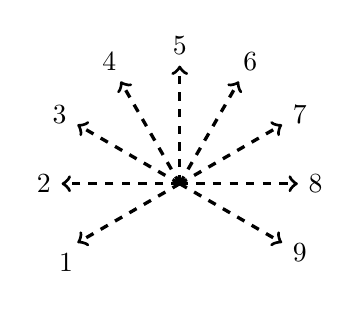
\begin{tikzpicture}
    \setfiguresize{-2.6}{-2.6}{+2.6}{+2.6}
    \begin{scope}
        \drawevenhexgrid{-2}{-2}{5}{5}
        \begin{scope}[dashed,very thick, ->]
            \draw (0,0) --   (90:1.5) node [anchor=270] {5};
            \draw (0,0) --   (60:1.5) node [anchor=240] {6};
            \draw (0,0) --   (30:1.5) node [anchor=210] {7};
            \draw (0,0) --    (0:1.5) node [anchor=180] {8};
            \draw (0,0) --  (330:1.5) node [anchor=150] {9};
            \draw (0,0) --  (210:1.5) node [anchor=60 ] {1};
            \draw (0,0) --  (180:1.5) node [anchor=0  ] {2};
            \draw (0,0) --  (150:1.5) node [anchor=330] {3};
            \draw (0,0) --  (120:1.5) node [anchor=300] {4};
        \end{scope}
        \drawaircraftcounter{0}{0}{90}{F-4}{}{}
     \end{scope}
\end{tikzpicture}
\end{fitheight}
\hfil
\begin{fitheight}{5.2\standardhexwidth}
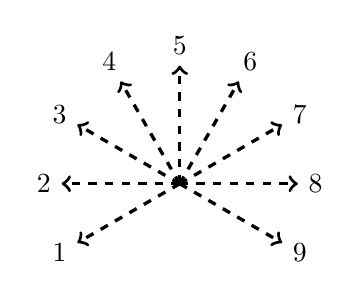
\begin{tikzpicture}
    \setfiguresize{-2.6}{-2.6}{+2.6}{+2.6}
    \begin{scope}[rotate=90]
        \drawevenhexgrid{-2}{-2}{5}{5}
        \begin{scope}[dashed,very thick,->]
            \draw (0,0) --   (0:1.5) node [anchor=270] {5};
            \draw (0,0) -- (330:1.5) node [anchor=240] {6};
            \draw (0,0) -- (300:1.5) node [anchor=210] {7};
            \draw (0,0) -- (270:1.5) node [anchor=180] {8};
            \draw (0,0) -- (240:1.5) node [anchor=150] {9};
            \draw (0,0) -- (120:1.5) node [anchor=30 ] {1};
            \draw (0,0) --  (90:1.5) node [anchor=0  ] {2};
            \draw (0,0) --  (60:1.5) node [anchor=330] {3};
            \draw (0,0) --  (30:1.5) node [anchor=300] {4};
        \end{scope}
        \drawaircraftcounter{0}{0}{0}{F-4}{}{}
    \end{scope}
\end{tikzpicture}
\end{fitheight}
\hfil
\begin{fitheight}{5.2\standardhexwidth}
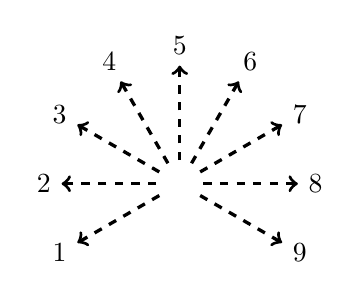
\begin{tikzpicture}
    \setfiguresize{-2.6}{-2.6}{+2.6}{+2.6}
    \begin{scope}[rotate=90]
        \drawevenhexgrid{-2}{-2}{5}{5}
        \begin{scope}[dashed,very thick,->]
            \draw   (0:0.3) --   (0:1.5) node [anchor=270] {5};
            \draw (330:0.3) -- (330:1.5) node [anchor=240] {6};
            \draw (300:0.3) -- (300:1.5) node [anchor=210] {7};
            \draw (270:0.3) -- (270:1.5) node [anchor=180] {8};
            \draw (240:0.3) -- (240:1.5) node [anchor=150] {9};
            \draw (120:0.3) -- (120:1.5) node [anchor=30 ] {1};
            \draw  (90:0.3) --  (90:1.5) node [anchor=0  ] {2};
            \draw  (60:0.3) --  (60:1.5) node [anchor=330] {3};
            \draw  (30:0.3) --  (30:1.5) node [anchor=300] {4};
        \end{scope}
        \drawaircraftcounter{-1}{0}{0}{F-4}{}{}
    \end{scope}
\end{tikzpicture}
\end{fitheight}

\figurecaption{figure:random-aaa}{Random Plotted AAA Fire}

\end{twocolumnfigure}
}


Some scenarios call for AAA to be fired randomly, or to be played solitaire. In these cases, AAA units fire only when determined by a die roll \changedin{1B}{1C-tables}{on the Random AAA Fire Tables as described below}{as described below and in Table \ref{table:random-aaa}}.

\paragraph{Aimed Fire.} Light and Medium AAA will always use random aimed fire in solitaire play.

Whenever an aircraft expends an FP in the range of an unfired AAA unit, roll one die. Check the result with the Random Fire Table and if a shot is indicated, resolve it via the normal AAA rules. The probability of a unit firing increases at closer ranges. Remember to check for each AAA unit separately and begin with the unit closest to the moving aircraft, then moving out to the next closest and so on. As long as AAA units remain to be fired, check for each subsequent aircraft that moves in range.

\paragraph{Barrage Fire.} Any non-AAA units capable of barrage fire are considered to use it all times.

\paragraph{Plotted Fire.} Heavy AAA will always use plotted fire. The target altitude and hex are determined randomly as follows in the Ground Unit Interaction Phase:

Start with the nearest aircraft to which the unit has a line of sight and which is sighted (if the AAA unit is equipped with an FCR, the aircraft does not have to be sighted). Roll the die once and consult \changedin{1B}{1C-tables}{the plotted fire direction diagrams}{Figure \ref{figure:random-aaa}} to determine the direction the plotted fire hex will be from the aircraft. A zero indicates the plotted hex is the aircraft's hex.

On any result other than a zero, roll the die again and halve the result dropping fractions to determine how many hexes in that direction the plotted fire hex lies.

To determine the altitude of the plotted fire; roll the die twice halving each result (drop fractions). Subtract the second result from the first. Add the target aircraft's start altitude for the current turn to the final result (+ or -) to get the altitude of the plotted fire. Repeat the procedure for each heavy AAA in play.

\section{Close Formation and AAA Fire}

Aimed AAA fire treats the whole close formation as a target. A minus one is applied to the too hit roll and if a hit occurs, randomly determine which aircraft takes the hit. When a hit does occur, the other aircraft in the formation must each roll a die and if a one results, they are also hit. Saving rolls apply and damage is resolved normally. Barrage and plotted fire attacks each aircraft normally.

\end{advancedrules}
